%
% A Real Chapter
\chapter{Background}
The 
% Modeling of Walking
\section{Modeling of Walking}
Different models have different limitations and advantages. Identifying the differences is important to develop an insight on how height variation can influence the system dynamics of a walking robot.
% lip
\subsection{Linear Inverted Pendulum Model}
In modeling of walking, a common approach is the modeling of the legs as a \acf{LIP}, as for example in \cite{kajita20013d}. Besides this, a not-linearized inverted pendulum is also widely used in the modeling of walking \cite{kuo2005energetic}.
In the \ac{2D} \ac{LIP} equations of motion, the motion of the tip along the $x$-axis does not affect the pendulum length $l$:
\begin{equation}
\ddot{x}=\frac{g}{l}x,
\label{eq:LIPeom}
\end{equation}
where $x$ the Cartesian x-coordinate of the pendulum tip and $\ddot{x}$ its acceleration.  At any position $x$, a local virtual straight pendulum can be considered, so this motion is at a constant height and $l=z_0$  holds. In \ac{3D} the system dynamics can be decoupled and the dynamics in $y$-direction read the same: $\ddot{y}=\frac{g}{l} y$. In \figref{fig:3dlip} this motion is visualized if the \ac{CoM} is relatively far from from the base. The pendulum base lies in the origin and $\cxy = [x,y]^T$ is the \ac{2D} \ac{CoM} projection on the horizontal plane. Because the \ac{LIP} assumption holds, the vertical component of the leg force $\boldsymbol{f}$ has to cancel out gravity acceleration: $f_z=mg$.\\
This decoupling of the system dynamics is one of the advantages of the use of a \ac{LIP} model. Taking for example a not-linearized inverted pendulum model, the dynamics of the pendulum tip in the $x$-direction are depending on both the $x$- and $y$-coordinate of the tip. Another advantage is that closed-form solutions exists for integrations over time of the model. This will be further explained in Section \ref{subsec:liporbit}.\\
\begin{figure}[h]
\centering
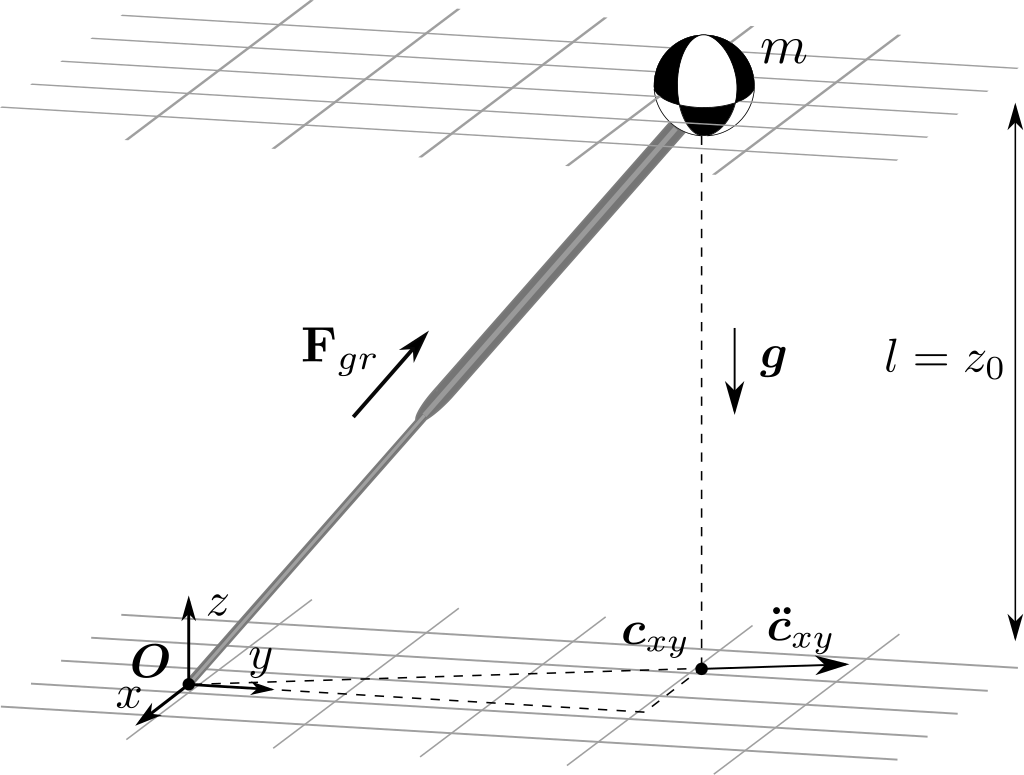
\includegraphics[width=0.5\textwidth]{STYLESTUFF/3DCoMwithoutfoot.png}
\caption{\ac{3D} motion of \ac{LIP} model.}
\label{fig:3dlip}
\end{figure}

% height var model
\subsection{Height Varying Models}
Models that are related to the \ac{LIP} model, but consider height variations are to be destinguished in two types: the inverted pendulum model, and a model with varying pendulum length. The inverted pendulum model is in human motion studies often used, as for example in \cite{kuo2005energetic}. The model with varying pendulum length is the most complicated of the three. Like described in the previous section, with the varying height models the dynamics of $x$- and $y$-direction become coupled. Also, a closed-form solution for time integration of the models does not directly exist. Attempts to closed-form expressions are discussed in Section \ref{subsec:nonorbit}. \\
In \figref{fig:2Dnonlinmodel} the varying length model is shown in \ac{2D}. The dynamics of the point mass can be written in two ways. One is as a function of the virtual leg force $\vect{f}$:
\begin{equation}
	m\ddot{x} = \vect{f}\frac{x}{\sqrt{x^2 + z^2}}.
	\label{eq:dynamicsprattstyle}
\end{equation}
The other one is as a function of the vertical acceleration $\ddot{z}$:
\begin{equation}
	\ddot{x} = \frac{g+\ddot{z}}{z}x.
	\label{eq:dynamicscaronstyle}
\end{equation}
Note that those models are identical, but can be used for different purposes.
\begin{figure}[h]
\centering
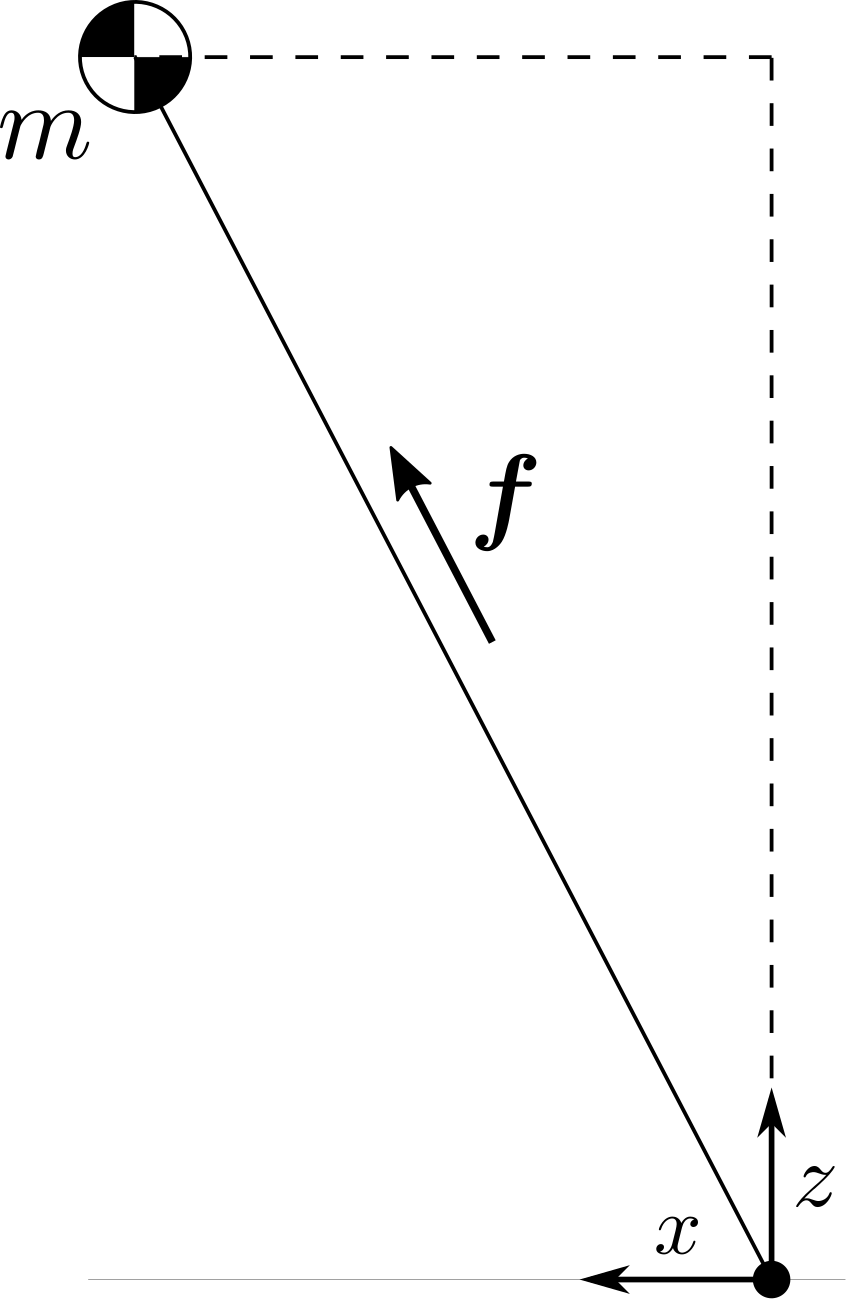
\includegraphics[width=0.2\textwidth]{STYLESTUFF/2Dnonlin.png}
\caption{Basic \ac{2D} inverted pendulum model with varying length.}
\label{fig:2Dnonlinmodel}
\end{figure}
% simple model
\subsection{Simple Walking Model}
The mentions of the above mentioned models of point-foot and point-mass type can be extended with adding a foot or feet, which the describe the support polygon. The support polygon plays an important role in the stability of the model. Next to this, the pendulum-type model can be extended with a body. In this thesis, a flywheel model is considered, where the combined effects of the dynamics of all other body parts are expressed as angular momentum around $\cxyz$.


% Ground Reference Points
\section{Ground Reference Points in Walking}\label{sec:grp}
A common approach for quantifying the dynamics of a walker, either a human or a robot, is the use of a \ac{GRF}, coming a from a single point of application on the ground. The magnitude and direction of the \ac{GRF} vector, the gravitational force vector, other external forces and the robots state determine the dynamics of the system. With the \ac{GRF} and the robots state, ground reference points can be derived, which can be used as a measure for the systems behavior.

% CoP
\subsection{The Center of Pressure}
The feet attached to the \ac{LIP} robot model increase the possibilities to control its motion. The ankles can apply a torque that would virtually move the position of the base of the inverted pendulum, so that the linear acceleration on the \ac{CoM} as in Eq. \eqref{eq:LIPeom} and the capture point as in Eq. \eqref{eq:cp} change. The new virtual base is called the \ac{CoP}. By its definition, this point only lives within the support polygon \cite{vukobratovic2004zero}. In \figref{fig:3dlipfoot} the definition of the \ac{CoP} is visualized. If the point mass is restricted to move on a constant height, the vertical component of $\boldsymbol{f'}$ counteracts gravity: $f'_z=g$. 

% ZMP
\subsection{The Zero Moment Point}
The \ac{ZMP} coincides during stable walking with the \ac{CoP}, like described in \cite{vukobratovic2004zero}. The two points however are not equal in unstable or more complicated cases, like falling over.  The \ac{CoP} is restricted to be in the support polygon, as this is a point that links to contact forces \cite{sardain2004forces}. The \ac{ZMP} however is not restricted to lie within the support polygon. The \ac{ZMP} is the point on the ground where the tipping moment equals zero. The tipping moment is defined as the component of the moment that is tangential to the ground surface. The \ac{ZMP} initially was introduced in \cite{vukobratovic1969contribution}.
\begin{align}
    x_{zmp}&=x-\frac{\fgrx}{\fgrz}z-\frac{\tau_y}{\fgrz}\\
    y_{zmp}&=y-\frac{\fgrz}{\fgrz}z+\frac{\tau_x}{\fgrz}
\end{align}

\begin{figure}[h]
\centering
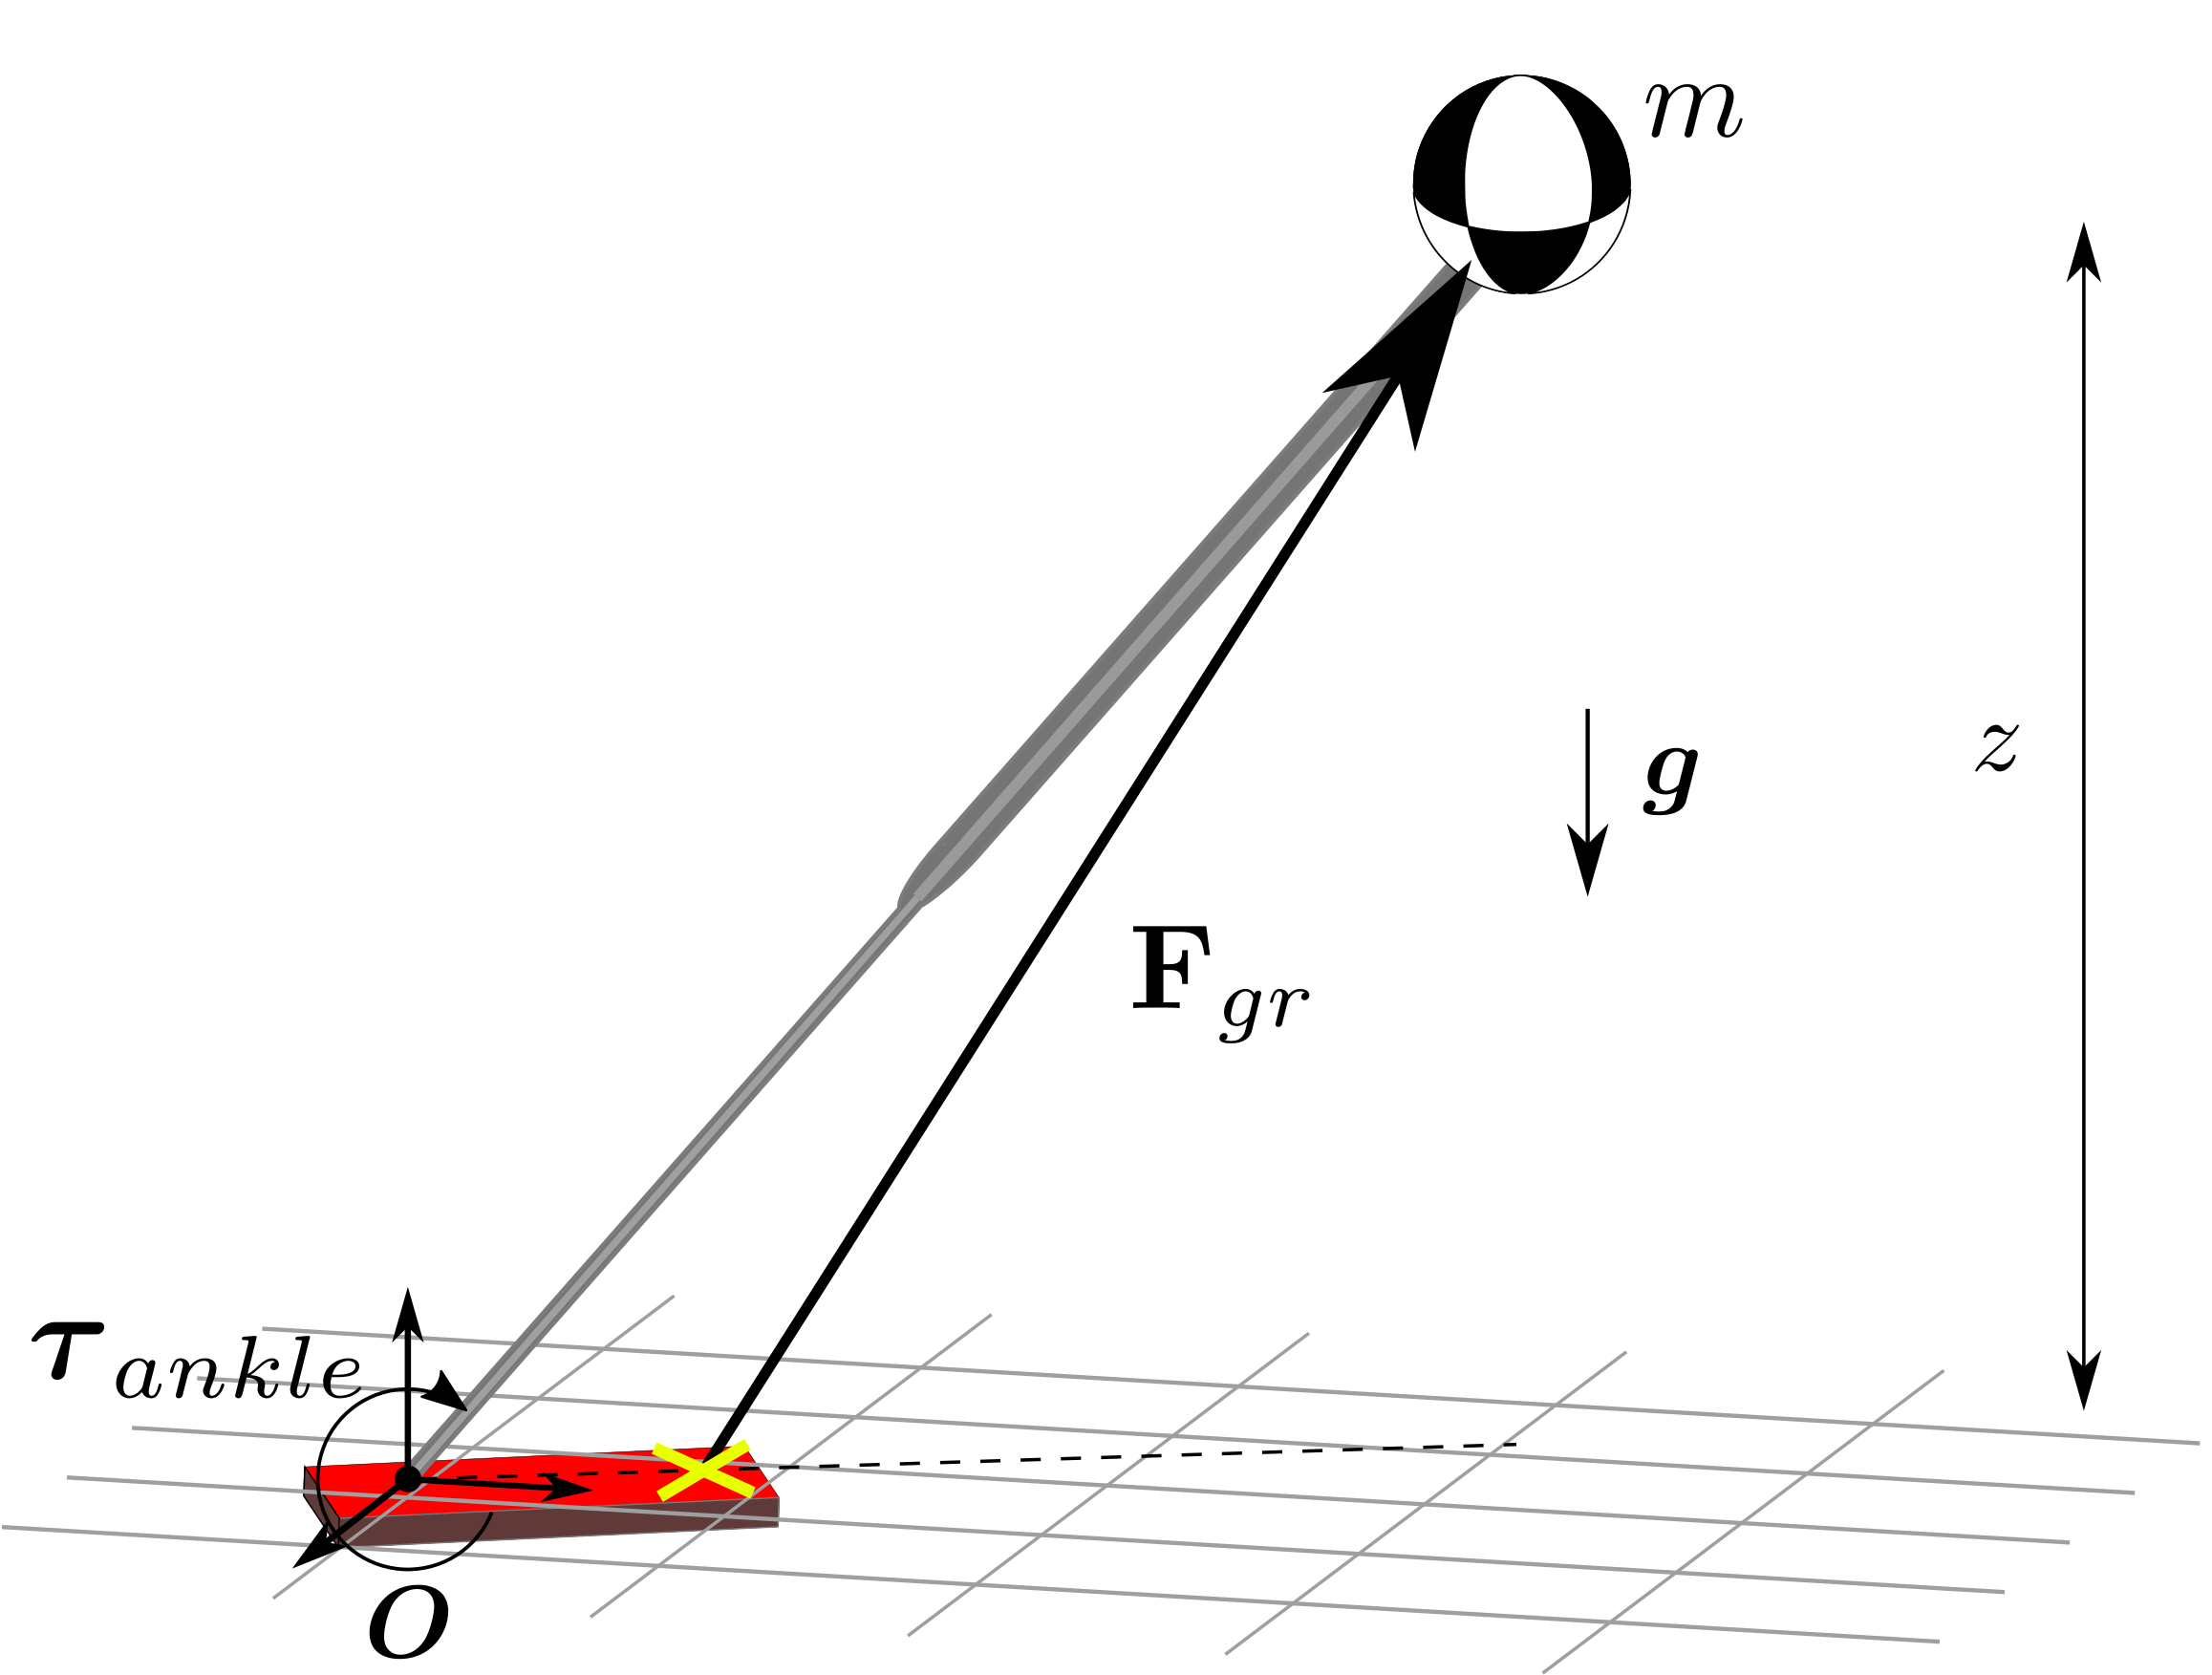
\includegraphics[width=0.5\textwidth]{STYLESTUFF/3DCoPviz.png}
\caption{\ac{3D} motion of \ac{LIP} model with foot. The yellow cross points out the \ac{ZMP} location.}
\label{fig:3dlipfoot}
\end{figure}

% CMP
\subsection{The Centroidal Moment Pivot}
The earlier mentioned points give sufficient measure for a \ac{LIP} model with point mass and finite-sized feet. However, any angular momentum applied by the body does not affect those points. In the case of the \ac{CoP} for example, the model assumes the resulting reaction force acts from the \ac{CoP} through the \ac{CoM}. The \ac{CMP} takes angular momentum into account, which can be used as a measure and for control \cite{popovic2005ground}. This is defined as the point where a line passing through the \ac{CoM}, parallel to the ground reaction force intersects with the ground surface. The \ac{CMP} is defined as
\begin{align}
    x_{cmp}&=x-\frac{\fgrx}{\fgrz}z\\
    y_{cmp}&=y-\frac{\fgrx}{\fgrz}z
\end{align}
where $\tau_{CoM}$ is the torque around the \ac{CoM}, $[x_{ZMP},y_{ZMP}]$ the \ac{ZMP} location on the horizontal plane and $F_{gr,z}$ is the ground reaction force in z-direction in Cartesian space. In \figref{fig:3dlipfootinertia} is displayed how body angular momentum affects the ground reaction force $\boldsymbol{f'}$ from the \ac{CoP} and how the \ac{CMP} can be determined with the intersection of a parallel line through the \ac{CoM} and the ground plane. For clarity the point in the image lies on the line from $\boldsymbol{O}$ to $\boldsymbol{x}$. This has not to be the case however, as the body can exert angular momentum along all axes. 
\begin{figure}[h]
\centering
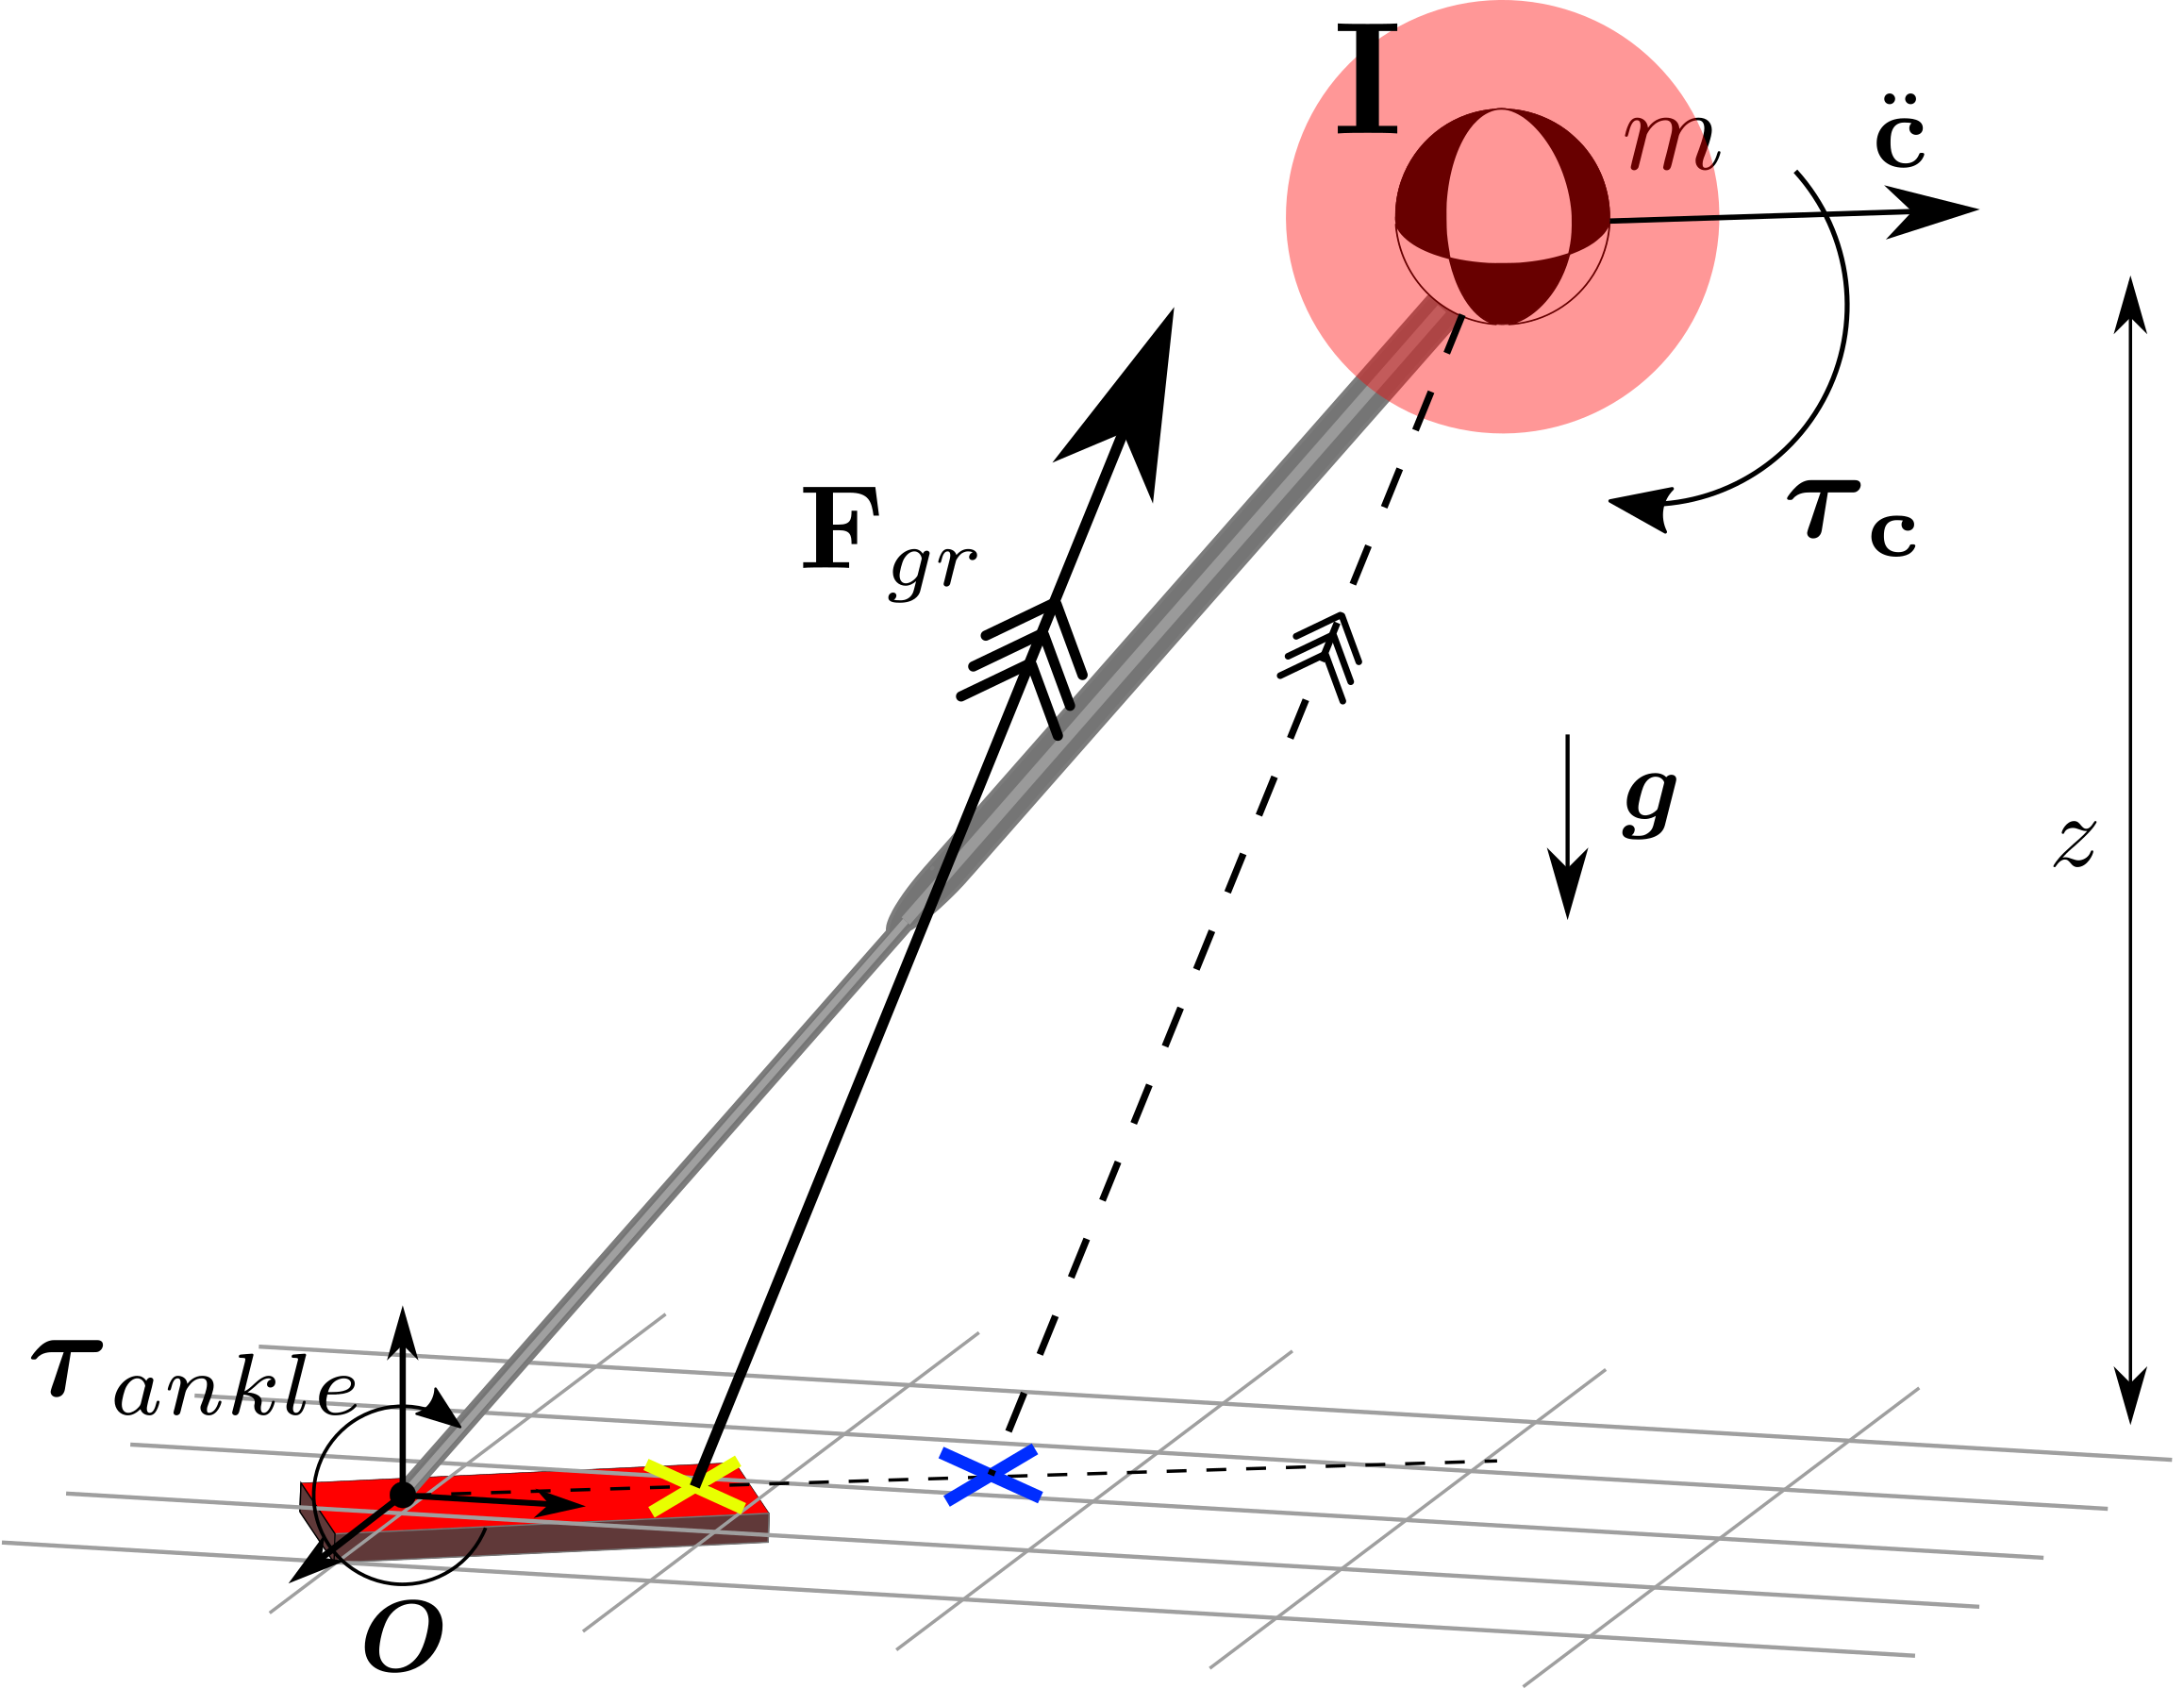
\includegraphics[width=0.5\textwidth]{STYLESTUFF/3DCMPCoPviz.png}
\caption{\ac{3D} motion of \ac{LIP} model with foot and body inertia. The blue cross points out the \ac{CMP} location.}
\label{fig:3dlipfootinertia}
\end{figure}
[MAKE IMAGES FOR ZMP AND CMP WITHOUT HEIGHT FIXED, AND SAY ZMP SUBSTRACTED ANG MOMENT]


% Energy of Walking
\section{Energy of Walking \& Capture}\label{sec:ewalking}
Knowing the system description of the pendulum-based model alone with its virtual base, a ground reference point, is not yet sufficient to know the system behavior forward in time. To have an indication of the state on a future moment in time, a form of energy of the system can be derived. With this energy can for example be determined whether or not the current state is stabilizable within the current footstep or coming footsteps: capturability \cite{koolen2012capturability}. 

% LIP orbital energy
\subsection{LIP Orbital Energy}\label{subsec:liporbit}
An early finding in an extended use of \ac{LIP} models can be found in \cite{kajita1992dynamic}. For the same reason that force is mass times acceleration: $F=ma$, impuse momentum is force times velocity: $I=Fv$ and the energy or work done by a force is the force times the distance, and thus the impulse integrated over the time interval: $E = Fs = \int Fv dt$, there can be reasoned that if one takes the time integral of the product of the second and the first derivative of a position, an expression for a normalized energy can be achieved: $\frac{E}{m}=\int av dt$. In the mentioned publication that same action is applied on Eq. \eqref{eq:LIPeom}:
\begin{equation}
\int (\ddot{x}-\frac{g}{l}x)\dot{x} dt = \frac{1}{2}\dot{x}^2-\frac{g}{2z_0}x +C=0
\label{eq:Elip}
\end{equation}
with $C$ the integration constant. The \ac{LIP} orbital energy is defined as $E_{LIP}=-C$. If $E_{LIP}>0$, the point mass will cross the $x$ position of the pendulum base with its current velocity. If $E_{LIP}<0$, the point mass will not cross the pendulum base and will have a turning point where the velocity becomes zero.

% ICP
\subsubsection{The Instantaneous Capture Point}
Although the finding of the \ac{LIP} orbital energy was crucial, more than a decade later \cite{pratt2006capture} introduced the \ac{CP}. Taking $E_{LIP}=0$ and taking the square root of Eq.  \eqref{eq:Elip} gives
\begin{equation}
x_{cp}=\sqrt{ \frac{z_0}{g}}\dot{x} 
\label{eq:cp}
\end{equation}
where $x_{cp}$ is the \ac{CP}, measured from the current pendulum tip position, based on the current tip velocity $\dot{x}$. This is the point where the velocity is exactly driven to zero and the pendulum is upright, where neither crossing of the pendulum base ocurred nor turning of body velocity. In \figref{fig:2dicp} a \ac{2D} visual explanation is given of this point.
\begin{figure}[h]
\centering
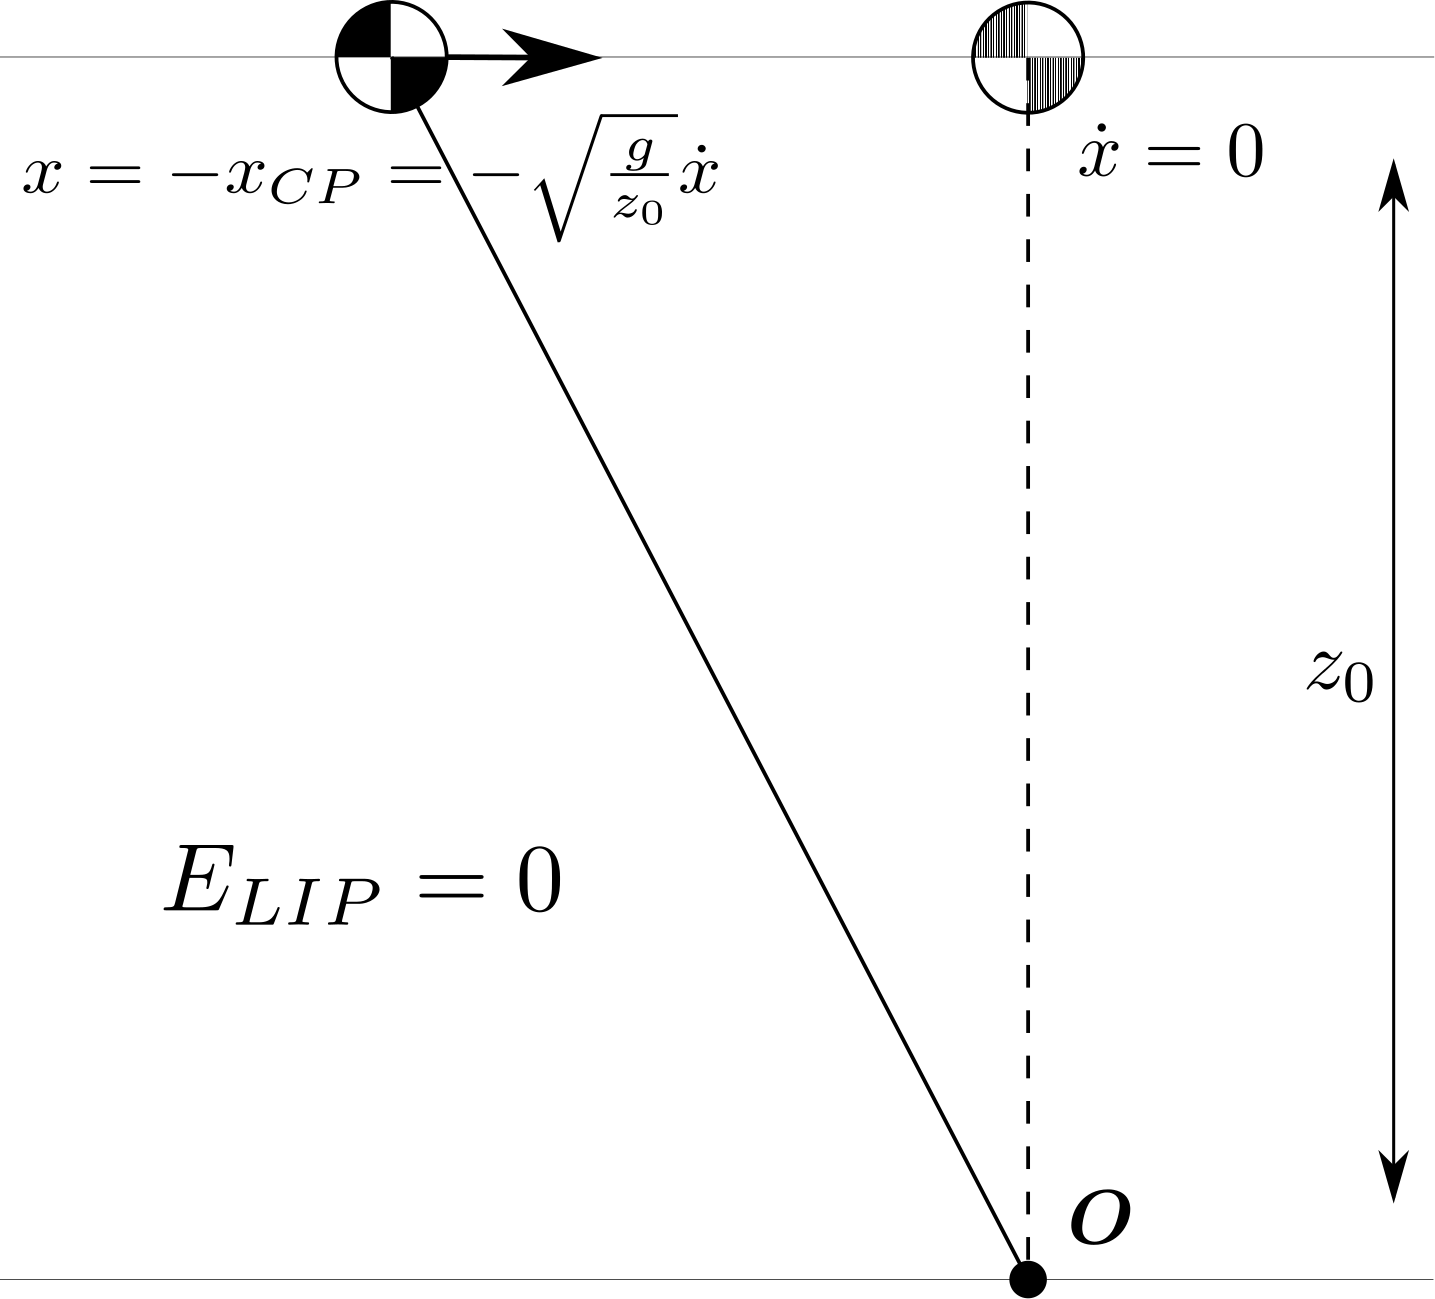
\includegraphics[width=0.4\textwidth]{STYLESTUFF/2DICP.png}
\caption{Visualization of path and states by the capture of the point mass according \ac{ICP} theory.}
\label{fig:2dicp}
\end{figure}
Later, the \ac{ICP} was introduced \cite{koolen2012capturability}, which gives a slightly different discription of the point:
\begin{equation}
\icpx=x+\sqrt{ \frac{z_0}{g}}\dot{x} 
\label{eq:icp}
\end{equation}
where $\icpx$ is the \ac{ICP}. In this way, the point can be described in the environment coordinates.
The $x$- and $y$-coordinate can be decoupled as in the equations of motion of Eq. \eqref{eq:LIPeom}. However, in the \ac{2D} horizontal plane, convergence to the capture point in one direction does not also include convergence to the capture point in the other. The direction of motion in \ac{3D} can also be directed not towards the pendulum base. Other similar mentions as the \ac{ICP} are extrapolated center of mass \cite{hof2008extrapolated} and the \ac{DCM} as described in \cite{takenaka2009real}. [LAAT  EVENTUEEL DECOUPLING DYNAMICS ZIEN]

% ICP dynamics
\subsubsection{\ac{ICP} Dynamics}
Because the ankle is not always located at the same location as the \ac{ICP} for the current horizontal velocity, for modeling and planning the time derivative is taken of the \ac{ICP}, which is named the \ac{ICP} dynamics \cite{koolen2012capturability}. This time derivative can be written as a function of the current \ac{ICP} location:
\begin{equation}\label{eq:icpdyn}
\dot{\icp}=\sqrt{ \frac{g}{z_0}}(\icp-\rcmp)
\end{equation}
where $\boldsymbol{x}_{ICP}$ is the $xy$-vector of the \ac{ICP} location and assuming that the pendulum base is the origin.

% Boundedness
\subsubsection{Boundedness Condition}
The \ac{ICP} and its cousins give a measure for location where to step, to come to a stop. This is however based on the point-mass, poin-foot \ac{LIP} model and no finite-sized supportpolygon is considered. An addition of the effects of the feet on capture  are included in the boundedness condition \cite{lanari2014boundedness}. The boundedness condition approaches the capture problem from a perspective that the point-mass has to converge to zero velocity in finite time. The solution of $x_u$, a point that also coincides with the \ac{ICP}, reads as:
\begin{equation}
x_u(t,r) = e^{\omega_0(t-t_0)}x_u(t_0) -\omega_0 \int_{t_0}^t e^{\omega_0(t-\tau)}r(\tau)d \tau,
\end{equation}
where $r(t)$ is the trajectory described by the used ground reference point, the virtual base of the pendulum, which can be chosen dependent on modeling choices. The boundedness condition reads as follows, if the the future input $r(t)$ makes the system convergence, the following equality holds:
\begin{equation}
x_u(t_0) = \omega_0 \int_{t_0}^{\infty} e^{-\omega_0(\tau-t_0)}r(\tau)d \tau.
\end{equation}
The initial condition, which is equal to the \ac{ICP}, has to be related to $r(t)$ by this expression.

%nonlinear orbital
\subsection{Orbital Energy with Height Variation}\label{subsec:nonorbit}
Next to the \ac{LIP} orbital energy and its relatives, there also exist expressions that incorporate height variations of the point-mass to the energy formulation. Examples are the time-varying \ac{DCM}, the orbital energy under a virtual constraint and the height varying boundedness condition. These works are discussed in the next section, since they are highly related to the research of focus.

% 2D polynomial
\subsubsection{Virtual Constraint}
With the dynamical description of Equation \eqref{eq:dynamicsprattstyle}, an energy expression is formulated by introducing the virtual constraint $z=f(x)$ \cite{pratt2007derivation}. The virtual constraint allows for the integration over time to be only expressed in the variable $x$, instead of also being the dependent on time $t$. The final expression for this energy proposed in the work reads as:
\begin{equation}\label{eq:eorbit}
    E_{orbit}  = \frac{1}{2}\dot{x}^2\bar{f}^2(x)+gx^2f(x) - 3g\int_{x_0}^xf(\xi)\xi d\xi = \frac{1}{2}\dot{x}_0^2\bar{f}^2(x_0)+gx_0^2f(x_0),
\end{equation}
where $E_{orbit}$ is the orbital energy under the constraint of $z=f(x)$.

% boundedness
\subsubsection{Boundedness Condition with Varying Height}
A height varying version of the boundedness condition from \cite{lanari2014boundedness} is introduced in \cite{caron2018balance} . By having a time varying natural frequency of the pendulum $\omega(t)$, the model combines the boundedness condition with the approach from \cite{hopkins2014humanoid}, which will be discussed . By its nonlinearity, this form of the boundedness condition becomes hard to solve and its applications will be further discussed in Section \ref{subsec:heightbalance}.



% CoM Height Variation
\section{Related Works CoM Height Variation}\label{sec:relatedworksheight}
The works that specifically focus on height variation on a humanoid robot are dividable in different goals of improvement. 
%var height terrain
\subsection{Varying Height Terrain}
Probably the most common goal of investigating height variation is the improvement of the behavior of the robot over rough or un-flat terrain. Improving the behavior over un-even terrain can devided in two categories:
\begin{enumerate}
	\item Improving the control framework for unexpected changes in terrain.
	\item Improving the dynamical plan, based on the give terrain information.
\end{enumerate} 
The generation of a dynamical plan of a redundant robotic system is traditionally done based on the \ac{LIP} model with constant height. The control framework has to deal with any height variations in terrain, and therefore also in the \ac{CoM}. In other words: the dynamics of the robot or roughly know in advance, but not precisely.\\
An example of incorporating height variations in terrain in the dynamic planning problem can be found in \cite{englsberger2013three}. Additional reference points, similar to ground reference points as in \ref{sec:grp}, are designed and used for the a planning method. The drawback here is that still a linearized model is considered and the trajectories between footsteps for the dynamical plan are straight lines. Another work improved this aspect by introducing the time-varying \ac{DCM} \cite{hopkins2014humanoid}. However, a closed form solution using this method is not available anymore, as the used model is non-linear.
%natural behavior
\subsection{Mimic Natural Behavior}
Straight leg walking. MPC approach to optimize for \cite{brasseur2015robust}. Walking reference for straight legs and dynamics feasibility \cite{kajita2017biped}. Paper online gait generation with vertical \ac{CoM} motions in dynamic plan \cite{terada2007online}
\cite{you2016straight} \cite{griffin2018straight} and more..
%effect
\subsection{Effects of Height Variation}
Research that investigates the energetic influences of height variations and impacts, often human orientated.
\cite{kuo2005energetic} \cite{lee1998determinants} \cite{gao2017increase} and more..
\subsection{Control for Balance}\label{subsec:heightbalance}
Two publications that consider height variations as control input for balance:
\cite{koolen2016balance} \cite{caron2018capturability}
This is the focus in this thesis.\\
With the  orbital energy from \cite{pratt2007derivation} and (\eqref{eq:eorbit}), a \ac{MPC} method is made by Koolen et al. in \cite{koolen2016balance}. Describing the function $f(x)$ from \eqref{eq:eorbit} as a cubic polynomial, the four polynomial are calculated in this method by introducing four constraints on the trajectory. There is one constraint in the initial height, one constraint on the initial direction, on e constraint on the final height and one contraint on the conservation of the orbital energy as in \eqref{eq:eorbit}. The final horizontal position and velocity are respectively above the virtual point-foot or `ankle' and zero. Which makes this trajectory a capture-trajectory for a point-foot, point-mass model, since no angular momentum is considered and only a single foot location. Furthermore, as mentioned earlier, this orbital energy is in \ac{2D}.\\


% Control Framework IHMC
\section{Humanoid Robotics at IHMC}
To support the theory discussed in later experiments, in this chapter a brief background of humanoid robotics at IHMC is given. Almost all algorithms are written in Java and similutations are run in \ac{SCS}.
%robots
\subsection{Robots}
\begin{figure}[h]
\centering
  \begin{subfigure}{0.45\textwidth}
  \centering
  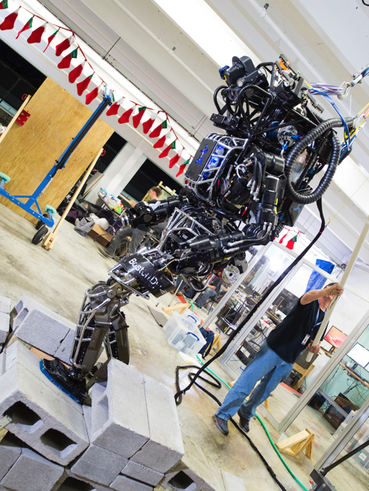
\includegraphics[width=.8\linewidth]{STYLESTUFF/AtlasOld.png}
   \caption{}
    \label{fig:atlas}
  \end{subfigure}
  \begin{subfigure}{0.45\textwidth}
    \centering
  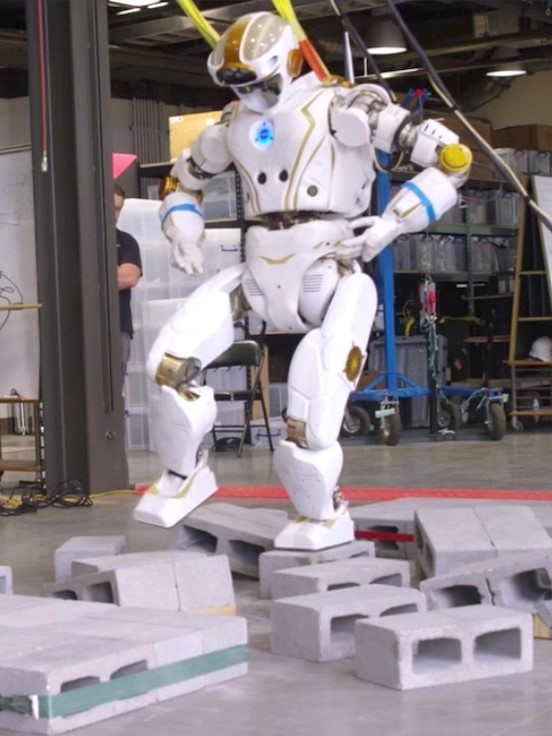
\includegraphics[width=.8\linewidth]{STYLESTUFF/Valkyrie.jpeg}
  \caption{}
   \label{fig:valkyrie}
  \end{subfigure}
  \caption{(a) Atlas and (b) Valkyrie walking over an un-even cinder block field at IHMC }
  \label{fig:robots}
\end{figure}
%walking states
\subsection{Walking States}
In contrary to running, with walking there is a state in every cycle with two feet in contact with the ground. This is the \ac{DS} state and the other state is called the \ac{SS} state. In \ac{SS}, the leg in contact with ground is the support leg and the foot taking a step is the swing leg. 
% planning
\subsection{Planning}
Planning of the robots motion in space is executed by seperating footstep planning from the generation of a dynamic plan. The dynamic plan is in this case an \ac{ICP} plan, but this is only one of the methods that exist in the field of research.
%footstepplan
\subsubsection{Footstep Planning}
A \ac{LiDAR} sensor on the head of the robot provides terrain information that is used for footstep planning. One way to generate a footstep plan is to let the user define it via a \ac{GUI}. Via relatively simple algorithmic checks on for example kinematic reachability, the \ac{GUI} can show whether a to be placed footstep is feasible or not. To make this process more autonomous, recently developments has been made in the creation of a footstep planner based on a A* search algorithm. 
%icpplanning
\subsubsection{ICP Planning}\label{subsec:icpplan}
Based on the footstep plan the dynamic plan, the \ac{ICP} plan is generated by using of solution of the linear differential equation the \ac{ICP} dynamics of \eqref{eq:icpdyn}:
\begin{equation}\label{eq:icpsol}
	\icp(t)=e^{\omega_0t}(\icp_0- \vect{r}) + \vect{r},
\end{equation}
where $\vect{r}$ is the virtual point-foot location, $\omega_0=\sqrt{\frac{g}{z_0}}$ is the natural frequency of the \ac{LIP} and $\icp_0$ is the initial \ac{ICP} location. This equation is only valid if the location of the virtual point-foot is assumed to be constant. The virtual point-foot depends on the model considered, but is typically the \ac{ZMP} or \ac{CoP} when no angular momentum is considered and the \ac{CMP} when an attempt is made to estimate the amount of angular momentum generated by the walking motion. Under the assumption of the constant virtual point-foot locations, multiple methods have been developed over the years and improvements are still going on. The most traditional generation of a \ac{ICP} reference trajectory is calulated with a single \ac{ZMP} knotpoint \cite{englsberger2012integration}. Using this method, for every footstep a single \ac{ZMP} knotpoint is used, and \ac{ICP} knotpoints $\icp_{0,n}$ for the $n$-th step are calculated by integrating the \ac{ICP} dynamics backwards in time for the footsteps considered. Using \eqref{eq:icpsol}, the local \ac{ICP} refence value can be computed at any time instance within the plan. \\
The above mentioned method is improved in \cite{englsberger2014trajectory}, where multiple \ac{CMP} knotpoints per foot are considered and \ac{SS} and \ac{DS} transitions are interpolated using splines. In the most recent improvements, continous \ac{CMP} reference trajectories are used for the generation of the \ac{ICP} trajectory \cite{seyde2018inclusion}. An estimate of the angular momentum generated during the walking motion is incorporated in the generation of the \ac{CMP} reference. At the time of writing, the latter method is the one currently in use, and which is used for the experiments in this thesis.
% icp control
\subsection{ICP Control}
From an \ac{CMP} and \ac{ICP} reference trajectory, the following control law is used to generate a desired \ac{CMP}:
\begin{equation}
    \rcmpd=\rcmpr + \mathbf{k}_{\xi}(\icp-\icpr),
\end{equation}
where $\rcmpd$ is the desired \ac{CMP}, $\rcmpr$ and $\icpr$ are the reference \ac{CMP} and \ac{ICP} from the \ac{ICP} planner respectively and $\icp$ is the current \ac{ICP}. From $\rcmpd$, the desired horizontal linear momentum rate of change can be computed:
\begin{equation}\label{eq:dotldxy}
    \dotldxy = \frac{\cxy-\rcmpd}{z_0}mg,
\end{equation}
where $\dotldxy$ is the desired horizontal linear momentum rate of change, which is basically the desired horizontal force. This value is send to the momentum-based control framework. 
% momentum control
\subsection{Whole-body Control \& Inverse Dynamics}
The desired horizontal linear momentum rate of change $\dotldxy$ from \ac{ICP} control is one of the inputs for the the whole-body \ac{QP}. The the solution of the whole-body \ac{QP} goes into a inverse dynamics solver, which calculates desired joint torques. 

\subsubsection{Centroidal Dynamics}
A fundamental part in robotics is to use the following mapping between joint velocities and end-effector motion:
\begin{equation}\label{eq:jacobian}
\matr{T}=\begin{bmatrix}\bs{\omega} \\ \bs{\upsilon} \end{bmatrix} = \matr{J}(\qjnt)\dqjnt \in \mathbb{R}^6,
\end{equation}
where $\dqjnt$ are the joint velocities, $\matr{J}(\qjnt)$ is the Jacobian that maps joint velocities to the end-effector twist $\matr{T}$. The twist consist of the angular velocity $\bs{\omega} \in \mathbb{R}^3$ and the linear velocity $\bs{\upsilon} \in \mathbb{R}^3$. In humanoid robotics, a fairly common approach is the use of centroidal momentum \cite{orin2013centroidal}:
\begin{equation}
\vect{h}=\begin{bmatrix}\vect{k} \\ \vect{l} \end{bmatrix} =\matr{A}(\qjnt)\dqjnt,
\end{equation}
 where $\matr{A}=\matr{I}\matr{J}$ is the inertia matrix $\matr{I}$ times the jacobian. The centroidal momentum $\vect{h}$ consists of the angular part $\vect{k}$ and the linear part $\vect{l}$. The time derivative of the centroidal momentum plays a crucial part in the control framework currently in use \cite{koolen2016design}:
\begin{equation}
\dot{\vect{h}}=\begin{bmatrix}\dot{\vect{k}}\\ \dot{\vect{l}} \end{bmatrix} =\matr{A}\ddot{\vect{q}} +\dot{\matr{A}}\dot{\vect{q}} = \matr{W}_g + \sum_i\matr{W}_{gr,i} + \sum_i \matr{W}_{ext,i}, 
\end{equation}
where $\matr{W}_g$ is the gravitational wrench and $\sum_i\matr{W}_{gr,i}$ the wrench exterted by \ac{GRF}. The other external wrenches, which can be caused for example by other contacts than ground, are considered zero in this thesis: $\sum_i \matr{W}_{ext,i}=\vect{0}$.
\subsubsection{Whole-body Quadratic Program}
The quadratic program, that translates momentum objectives, motion objectives and privileged configuration objectives to desired joint accelerations and desired \ac{GRF} is structured as follows:
\begin{equation}
\begin{array}{rlcl}
\displaystyle \min_{\bs{\ddot{q}}_d,\bs{\rho}} & \multicolumn{3}{l}{J_{\bs{\dot{h}}_d} + J_{\bs{J}} + J_{\bs{\rho}} + J_{\bs{\ddot{q}}_d}  + J_p} \\
\textrm{s.t.} & \matr{A}\ddqjntd + \dot{\matr{A}}\dqjnt = \matr{W}_g + \matr{Q}\bs{\rho}+\sum_i\matr{W}_{ext,i}\\
&\displaystyle \bs{\rho}_{min} \leq \bs{\rho}\\
&\ddot{\qjnt}_{min} \leq \ddqjntd \leq \ddot{\qjnt}_{max},
\end{array}
\end{equation}
where $\ddqjntd$ are the desired joint accelerations, $\matr{Q}\bs{\rho} = \sum_i\matr{W}_{gr,i}$ is the basis vector matrix $\matr{Q}$ times the basis vector multiplers $\bs{\rho}$. The minimum $\bs{\rho}_{min}$ has to be at least zero, because of the unilateral contact constraint of the robot. The total cost $J$ is composed of the following cost terms:
\begin{equation*}
\begin{array}{rlcl}
$Momentum objective cost:$ & J_{\dot{\vect{h}}_d}= \wght_{\dot{\vect{h}}_d}||\matr{A}\ddqjntd + \dot{\matr{A}}\dqjnt - \dot{\vect{h}}_d||^2\\
$Motion objective cost:$ & J_{\matr{J}_m} = \wght_{\matr{J}_m}||\matr{J}_m\ddqjntd-\vect{p}||^2\\
$Contact force cost:$ & J_{\bs{\rho}}=\wght_{\bs{\rho}}||\bs{\rho}||^2 \\
$Joint acceleration cost:$ & J_{\ddqjntd} = \wght_{\ddqjntd}||\ddqjntd ||^2 \\
$Privileged configuration cost:$ & J_p = \wght_p||(\matr{I} - \matr{J}_t^{\dagger}\matr{J}_t)\ddqjntd - \ddqjntp||^2,
\end{array}
\end{equation*}
where the weighting terms $\wght$ can have a selecting function as well. For example the centroidal momentum rate of change objective $J_{\dot{\vect{h}}_d}$ only consists of the linear part and is only affected by $\dotld$. The motion task jacobian $\matr{J}_m = [\bs{J}_1^T\quad...\quad\bs{J}_N^T]^T$ and objective vector $\vect{p} = [\vect{p}_1^T\quad...\quad\vect{p}_N^T]^T$ consist of all concatenated jacobians and objective values that map either joint acceleration to end-effector motion, as in Equation \eqref{eq:jacobian} or joint acceleration to joint joint acceleration. The motion objective values $\vect{p}$ consist of PD-controlled desired accelerations, coming for example from trajectory tracking of the swing leg or maintaining the upper-body orientation. The last cost term $J_p$ is determined by the privileged joint accelerations $\ddqjntp$. Here is the all$\bs{J}_t$ the all-task jacobian consisting of both $\matr{A}$ and $\matr{J}_m$. The damped Moore-Penrose pseudo-inverse  $\matr{J}_t^{\dagger} = \matr{J}_t^T(\matr{J}_t\matr{J}_t^T +\mu^2)^{-1}$ with $\mu>0$ is used in the null-space projector $(\matr{I} - \matr{J}_t^{\dagger}\matr{J}_t)$, which projects the priviliged acceleration objective in the null-space of the primary task jacobian $\matr{J}_t$. This can for example be used in singularity avoidance, where the priviliged accelerations can be used to determine the configurarion of the robotic chain.  
\paraskip
An important note considering the research goal is the generation of vertical \ac{CoM} motion of the robot. The desired linear momentum rate of change $\dotld$ consists, next to its horizontal component of Equation \eqref{eq:dotldxy}, of a vertical part:
\begin{equation}
\dotldz =m(k_p(z-z_r) + k_d\dot{z}), 
\end{equation}
where $k_p, k_d$ are the PD-control gains and $z_r$ is the reference height coming from a reference trajectory. Decision variables for this trajectory are for example kinematic reachability and height changes in terrain, but maintaining the robot's balance is \textit{not } a part of those decision variables.


\subsubsection{Inverse Dynamics}
Desired joint torques $\bs{\tau}_d$ are calculated via a revursive Newton-Euler inverse dynamics algorithm using solution of whole-body \ac{QP}: $\bs{\ddot{q}}_d$ and $\bs{\rho}$.
\begin{equation}
    \bs{\tau}_d = \matr{M}(\qjnt)\ddqjntd + \matr{C}(\qjnt,\dqjnt) + \matr{G}(\qjnt) + \matr{J}^T \vect{W},
\end{equation}
where the external wrench $\vect{W}$ is determined by, amongst other things, $\bs{\rho}$.

